\documentclass[tikz]{standalone}
\usetikzlibrary{decorations.markings}
\newcommand{\circo}{~\raisebox{1pt}{\tikz \draw[line width=0.5pt] circle(1.0pt);}~}
\begin{document}
    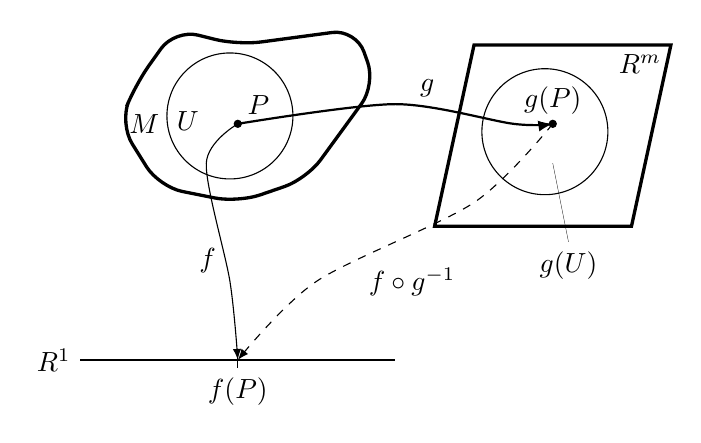
\begin{tikzpicture}[>=latex]
        \coordinate (a) at (0,0);
        \coordinate (b) at (4,0);
        \coordinate (c) at (0,-3);
        \draw (-2,-3) node[left] {$R^1$}--(2,-3) (0,-2.9)--(0,-3.1) node[below] {$f(P)$};
        \draw[dashed,->,postaction={
            decorate,
            decoration={
                markings,
                mark=at position 0.6 with \coordinate (x);
            }
        }] plot[smooth] coordinates {(b) (3,-1) (1,-2) (c)};
        \draw (x) node[below right] {$f\circ g^{-1}$};
        \draw[->,postaction={
            decorate,
            decoration={
                markings,
                mark=at position 0.6 with \coordinate (y);
            }
        }] plot[smooth] coordinates {(a) (-.4,-.5) (-.1,-2) (c)};
        \draw (y) node[left] {$f$};
        \draw[thick,->,postaction={
            decorate,
            decoration={
                markings,
                mark=at position 0.6 with \coordinate (z);
            }
        }] plot[smooth] coordinates {(a) (2,.25) (3.5,0) (b)};
        \draw (z) node[above] {$g$};
        \fill (a) circle (1.5pt) node[above right] {$P$} (b) circle (1.5pt) node[above] {$g(P)$};
        \draw (-.1,.1) circle (0.8) ++(185:0.8) node[right] {$U$};
        \draw[very thick,rounded corners=3mm] (-1.5,0)--(-1.3,.5)--(-.8,1.2)--(0,1)--(1.5,1.2)--(1.75,.5)--(0.875,-.7)--(0,-1)--(-1,-.8)--cycle;
        \draw (-1.5,0) node[right] {$M$};
        \draw (3.9,-.1) circle (0.8);
        \draw[very thick] (3,1)--(5.5,1)--(5,-1.3)--(2.5,-1.3)--cycle;
        \draw (5.5,1) node[below left] {$R^m$};
        \draw[ultra thin] (4,-.5)--++(.2,-1) node[below] {$g(U)$};
    \end{tikzpicture}
\end{document}